\section{Histoire cas}

\begin{frame}{Histoire de cas}
	\centering
	\begin{columns}
		\column{0.49\textwidth}
		\begin{itemize}
			\item Homme de 68 ans
			\item Fibrose pulmonaire idiopathique
			\item Greffe pulmonaire unilatérale
			\item Embolie pulmonaire, sepsis...
			\item Réintubé pour bronchoscopie
		\end{itemize}
		\column{0.49\textwidth}
	\centering
			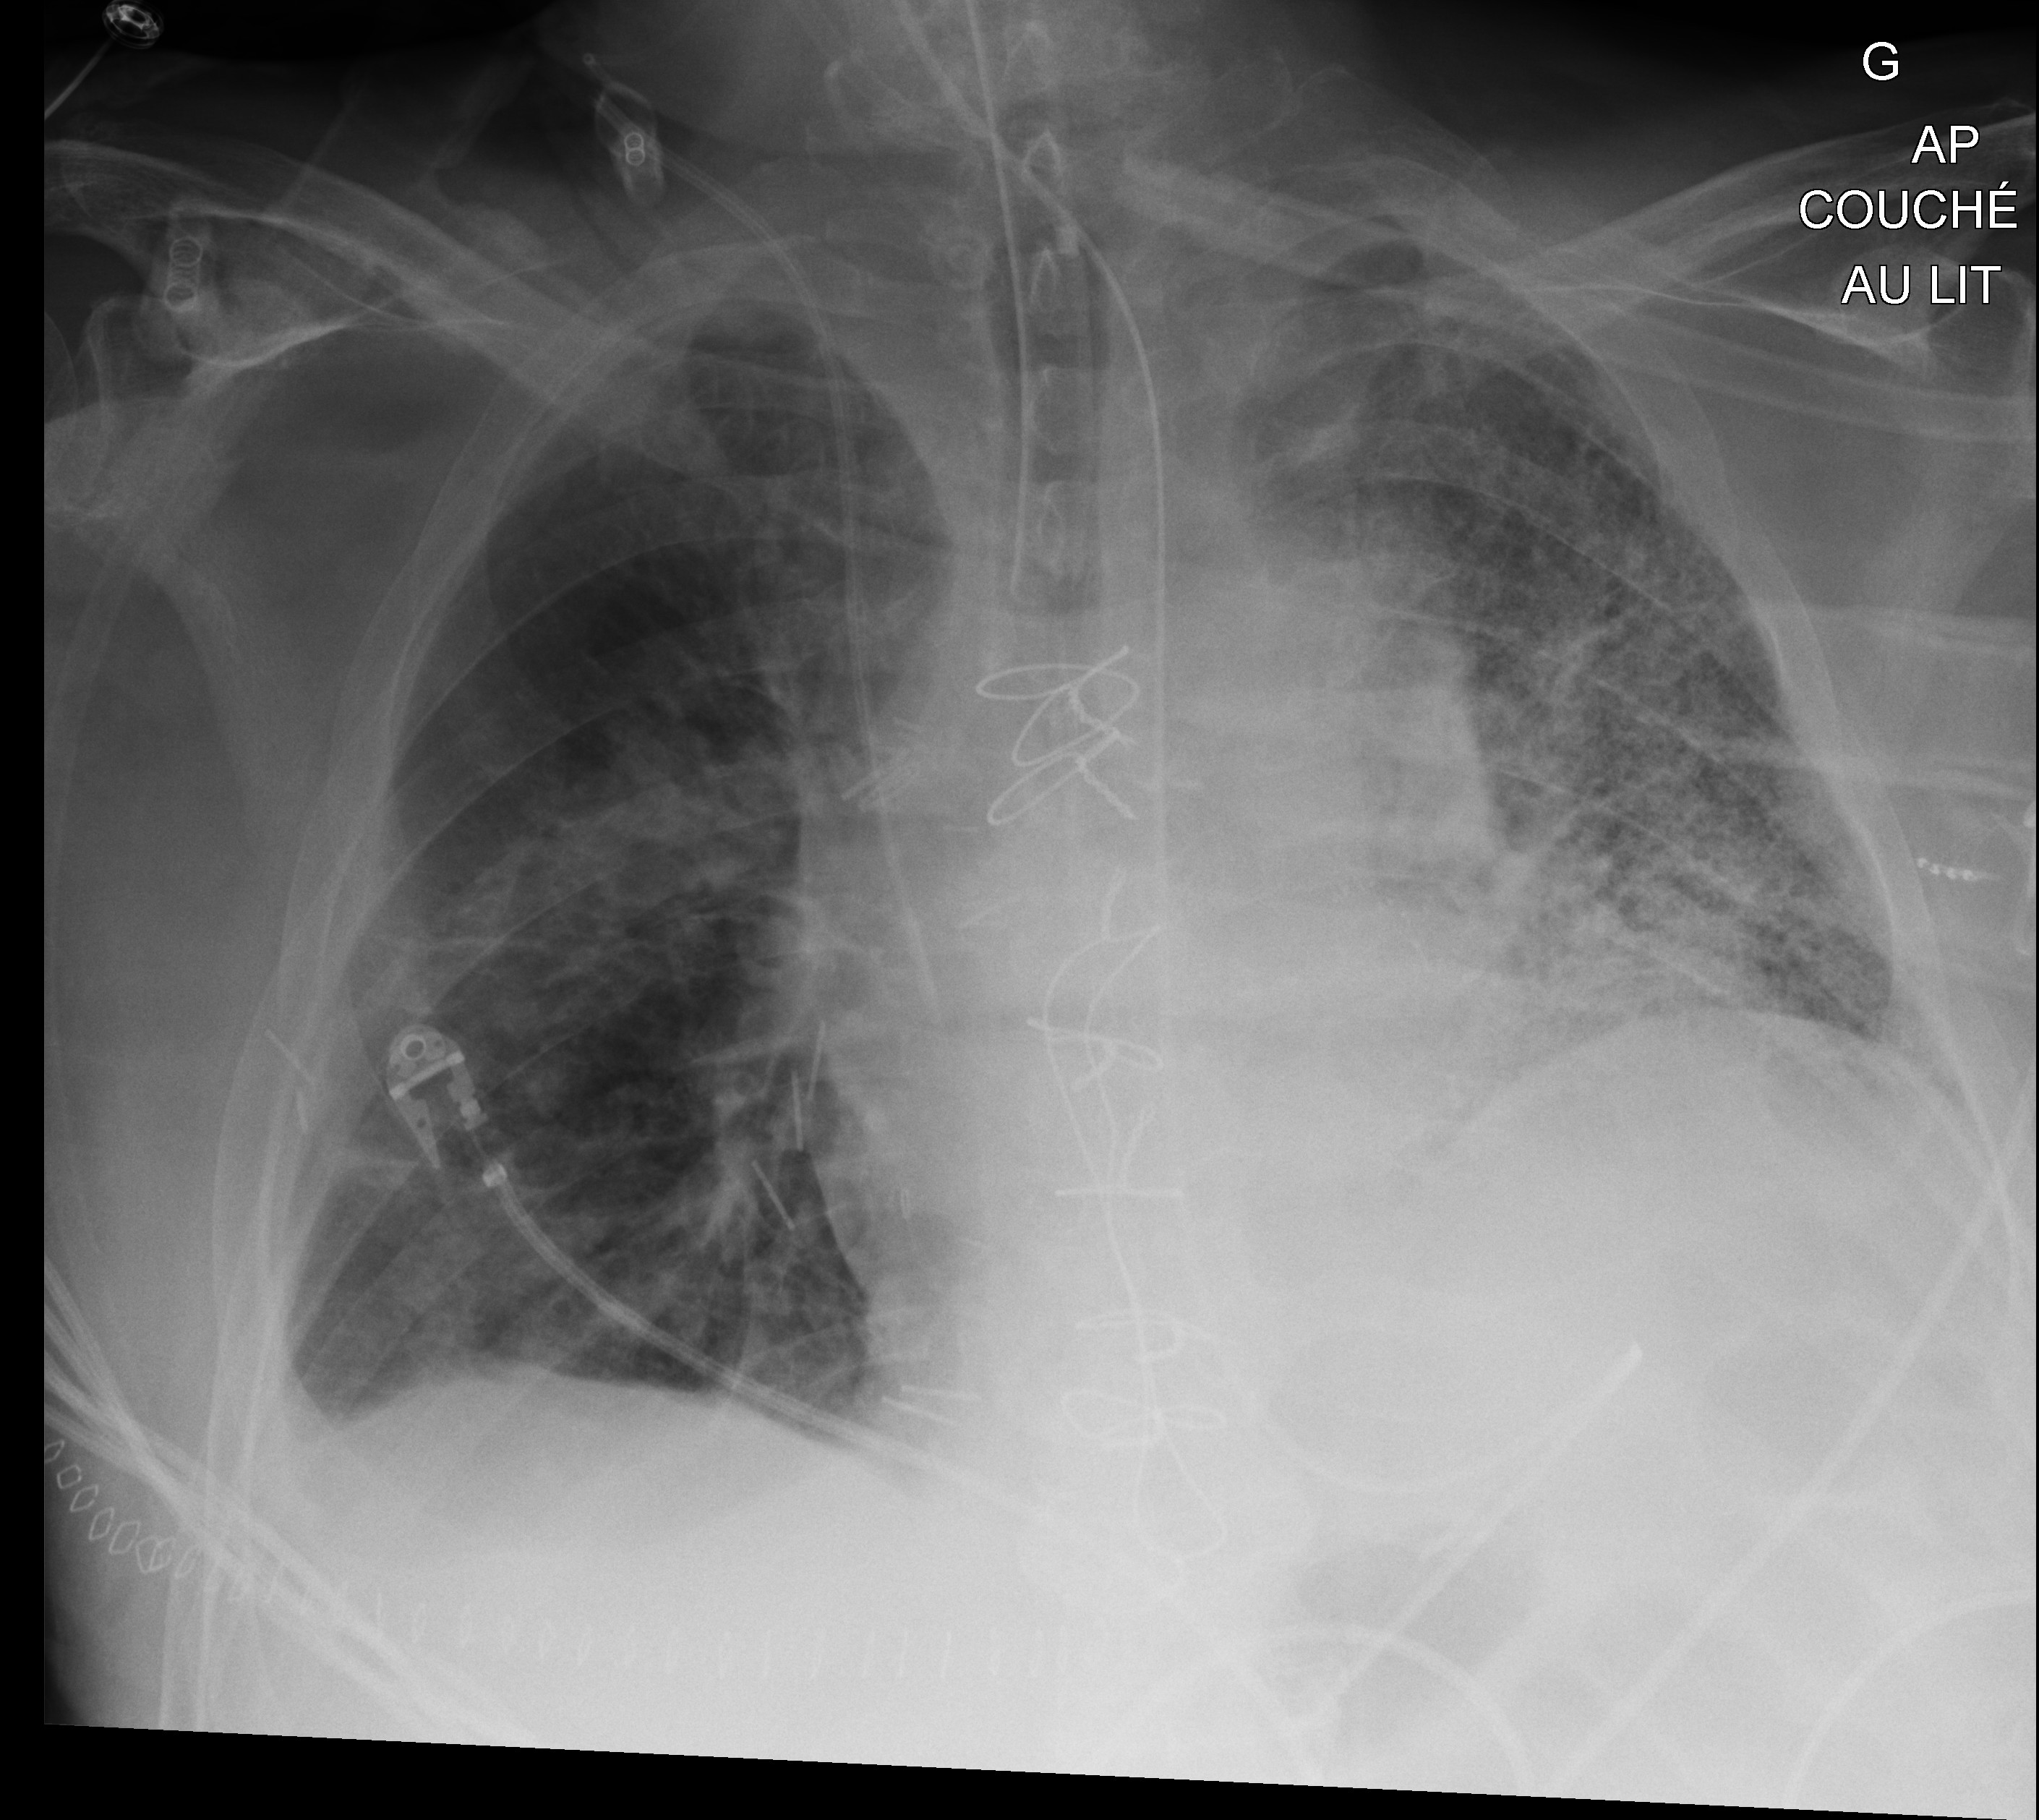
\includegraphics[
			width=\textwidth,
			trim=200 250 0 0,
			clip
			]{radiographies/23marsPM.jpg}
\end{columns}
\end{frame}

\begin{frame}
	\centering
	\begin{tikzpicture}
		\node[inner sep=0] (R) { 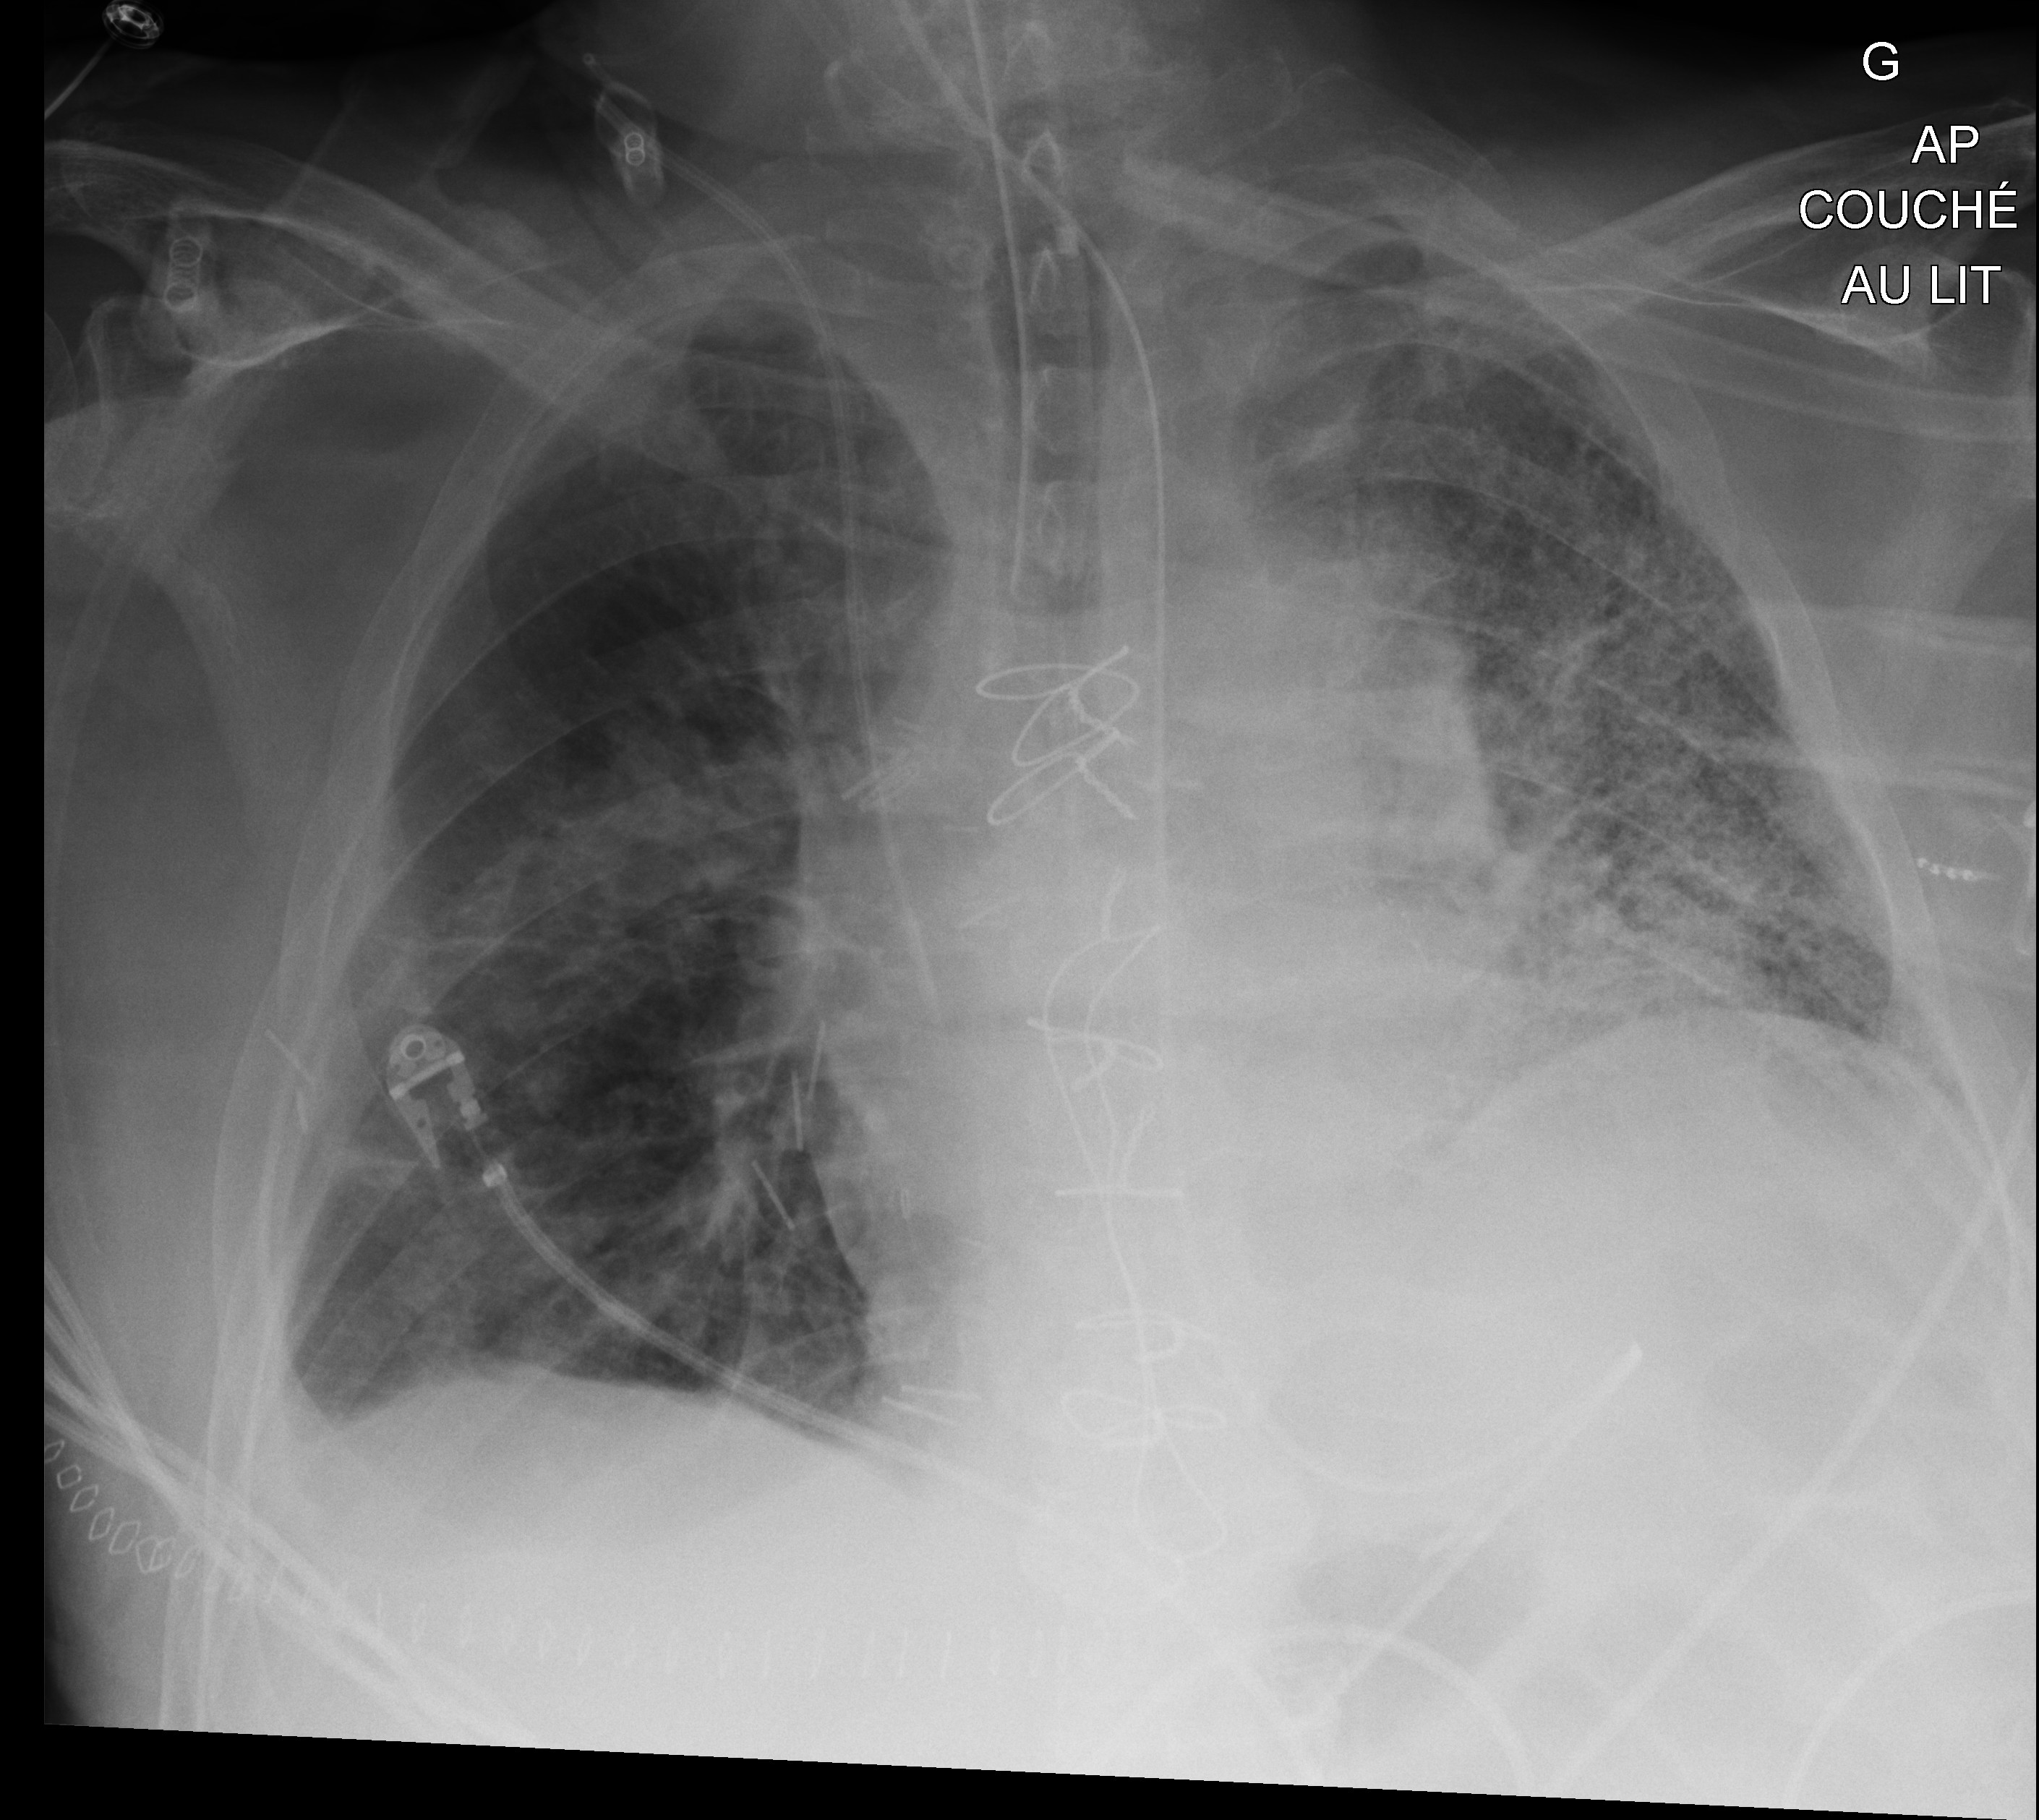
\includegraphics[
			height=\paperheight-1mm,
			trim=200 250 0 0,
			clip
			]{radiographies/23marsPM.jpg}
		};
		\end{tikzpicture}
\end{frame}

%%%%%%%%%%%%%%%%%%%%%%%%%%%%%%%%%%
% Chronologie                    %
%%%%%%%%%%%%%%%%%%%%%%%%%%%%%%%%%%

\begin{frame}{Chronologie}
	\centering

	\begin{tikzpicture}[
		xscale=0.4,
		pin distance=9mm,
		every node/.style={
			fill,
			circle,
			inner sep=1.5pt
		},
		every pin/.style={
			rectangle,
			text=bleuclairchum,
			fill=none
		},
		grad/.style={
			fill=none,
			label=below:j.\,\x,
			font=\tiny
		}
		]

		\draw [->](-1, 0) -- (29, 0);

		\begin{scope}[
			fill=bleuclairchum
		]
		\node [pin=Greffe pulmonaire, label=below:j.\,0] at(0, 0) {};
		\node [pin=below:Extubation, label=above:j.\,1] at(1, 0) {};
		\node [pin=Intubation, label=below:j.\,11] at(11, 0) {};
		\node [pin=below:Extubation, label=above:j.\,15] at(15, 0) {};
		\node [pin=Intubation, label=below:j.\,22] at(22, 0) {};
		\node [pin=below:Découv. autocécl., label=above left:j.\,25] at(25, 0) {};
		\node [pin={[text=red]below:Découv. autocécl.}] at(25, 0) {};
		\node [pin={[pin distance=1.5cm]Extubation}, label=below right:j.\,26] at(26, 0) {};
	\end{scope}
	\end{tikzpicture}

\end{frame}
%%%%%%%%%%%%%%%%%%%%%%%%%%%%%%%%%
% Captures d'écran              %
%%%%%%%%%%%%%%%%%%%%%%%%%%%%%%%%%

\begin{frame}
	\centering
	\begin{tikzpicture}[
		spy using outlines={circle,
      magnification=4,
			connect spies
		},
		servoucell/.append style={
			fill=black!80,
			text=white, 
			transform shape,
			scale=0.5
		}
	]
	\node [inner sep=0] (img) {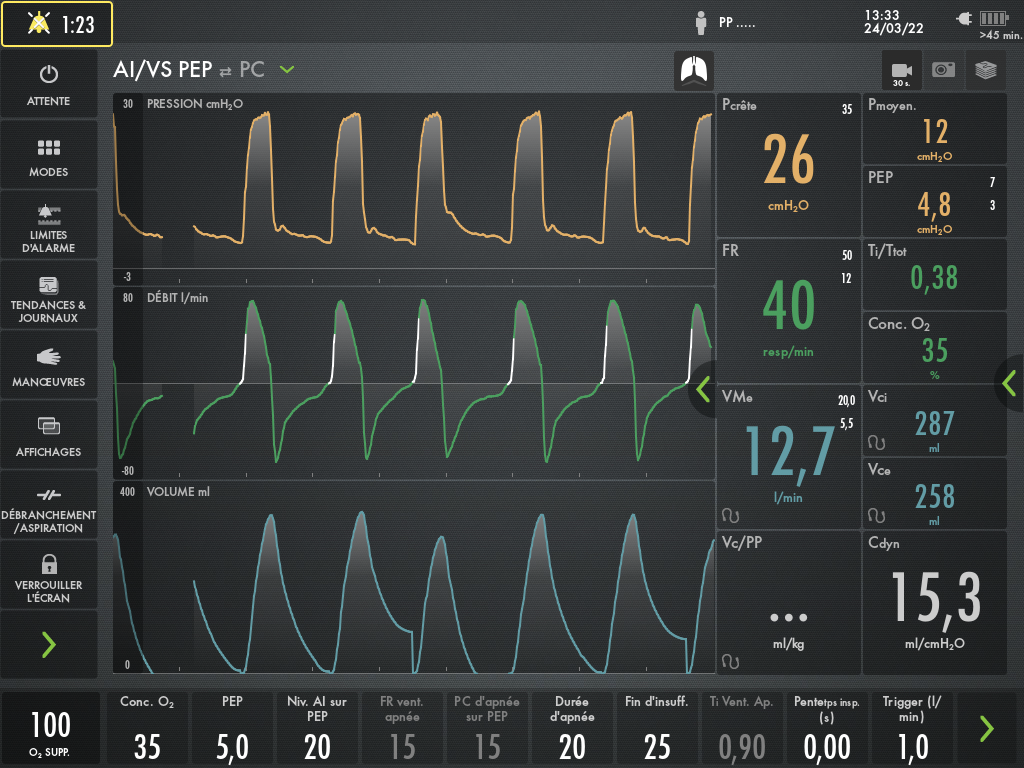
\includegraphics[height=\pageheight]{captures/220324_133316.png}};
	\only<2>\spy[red, size=3cm] on (-.2,0) in node at (2,2);
	\only<3>\spy[red, size=3cm] on (-.1,1.8) in node at (-3,2);
\node<4>[servoucell, anchor=west] at(img.east){
		\nodepart{one}P0.1
			\nodepart[font=\Huge]{two}0.2
				\nodepart{three}cm\,H\scalebox{.75}{2}O
				};
	\end{tikzpicture}
\end{frame}


\begin{frame}
	\centering
			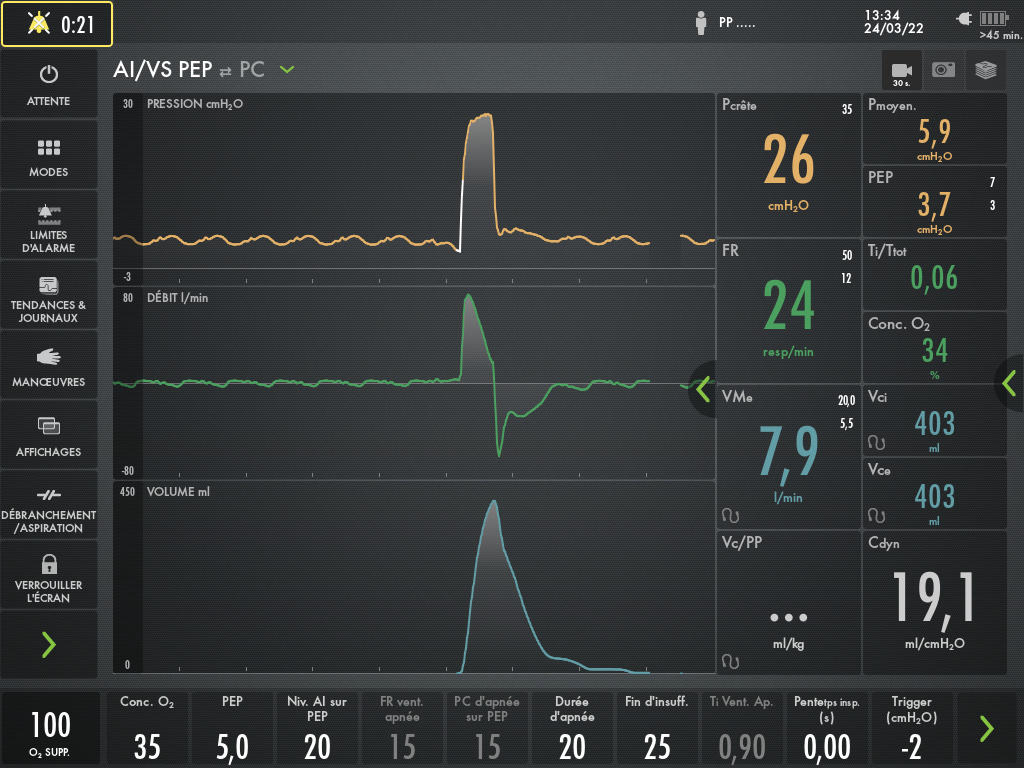
\includegraphics[height=\pageheight]{captures/220324_133418.png}
\end{frame}

\begin{frame}
	\centering
	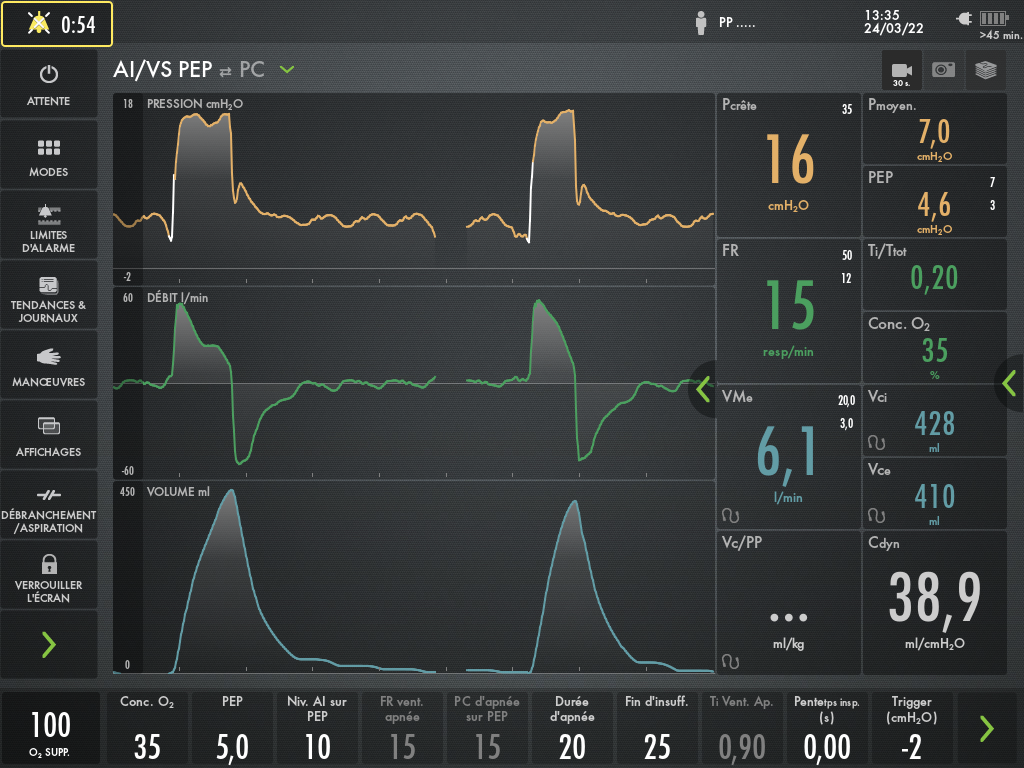
\includegraphics[height=\pageheight]{captures/220324_133546.png}
\end{frame}

